\documentclass[12pt]{article} %aqui fala o tipo de documento e o tamanho da fonte. Opções: tamanho do texto (10pt, 12pt, 14pt), formato do papel (a4paper, a5paper, b5paper, letterpaper, legalpaper, executivepaper), o número de colunas (onecolumn, twocolumn), entre outras opções.
%Por exemplo, [12pt,a4,twocolumn].
%classe: article, report, letter, book ou slides. Instalar abnt para quem está pensando no tf
\usepackage[brazil]{babel} %hifenização em português do brasil

\usepackage[T1]{fontenc} % caracteres com acentos são considerados um bloco só
\usepackage{ae} %arruma a fonte quando usa o pacote acima
\usepackage[utf8]{inputenc}
\usepackage{graphicx}%Para inserir figuras


\begin{document} % Aqui começa o documento
\title{Tutorial RS-232 da placa DE2-115 da Altera\vspace{3.5cm}} % título

\author{
	Gustavo de Faria Silva
	\texttt{gustavofaria@ufu.br}
	\and
	João Paulo de Oliveira
	\texttt{joaopaulodeoliveira123@gmail.com}
	\and
	Lucas Rossi Rabelo
	\texttt{lucasrossi98@hotmail.com}
	\vspace*{10cm}
}

% * <joaopaulodeoliveira123@gmail.com> 2017-11-23T13:53:11.198Z:
%
% ^.
\maketitle %cria o título

%\def \negritovi {\textbf} %Criando comandos

\tableofcontents %índice
\pagebreak % Quebra de página
%\listoffigures %indice de fig%uras
%\listoftables %indice de tabelas
%\pagebreak % Quebra de página
\section*{Caracteŕisticas físicas e elétricas}
O RS-232 na Placa DE2-155 da Altera oferece um conector Db-9 fêmea para fazer o interfaceamento com o computador ou outro dispositivo de comunicação. Um computador conectado com a placa deve ter as seguintes configurações:
\begin{itemize}
	\item \bf{Taxa de transfêrencia:} 115200
    \item \bf{Bit de paridade:} Nenhum
    \item \bf{Bits de dados:} 8
    \item \bf{Bit de parada:} 1
    \item \bf{Controle de fluxo:} ON
\end{itemize}
A DE2-115 usa o transceptor ZT3232 para gerenciar a conexão entre a placa. Para mais detalhes sobre o transceptor, consulte o datasheet. 

\begin{figure}[!h]
\centering
	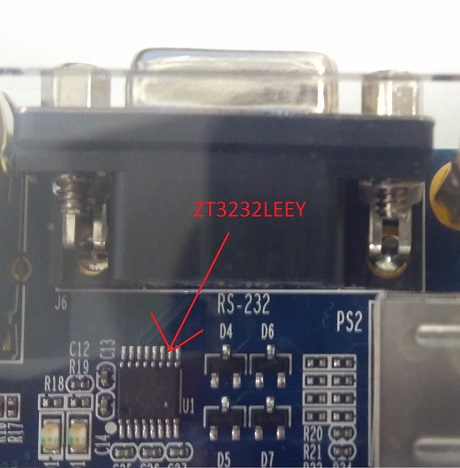
\includegraphics[scale=0.5]{imagens/IMG_20171123_110859}
	\caption{CI utilizado para o RS-232}
	\label{Rotulo}
\end{figure}

\begin{figure}[!h]
\centering
	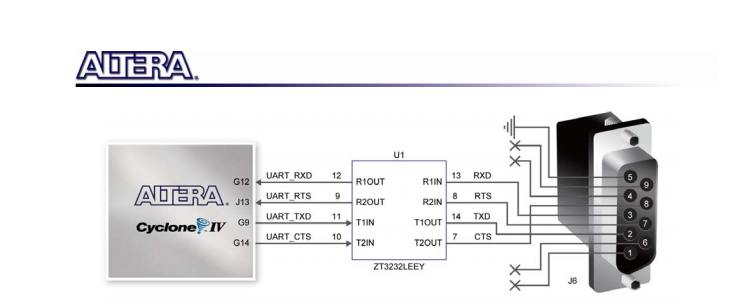
\includegraphics{imagens/conex_o.png}
	\caption{Pinagem utilizada entre o FPGA e o ZT3232LEEY}
	\label{Rotulo}
\end{figure}


\begin{table}
\centering
\caption{Tabela de associação de pinos}
\label{pin_assignment}
\begin{tabular}{|l|l|l|l|}
\hline
Signal Name & FPGA Pin No & Descrição                      & Voltagem \\ \hline
RXD         & PIN\_G12    & Receptor da UART               & 3.3V     \\ \hline
TXD         & PIN\_G9     & Transmissor da UART            & 3.3V     \\ \hline
CTS         & PIN\_G14    & Limpar para enviar na UART     & 3.3V     \\ \hline
RTS         & PIN\_J13    & Requisição para enviar na UART & 3.3V     \\ \hline
\end{tabular}
\end{table}


\section*{Handshake}
\section*{Uarts}
\section*{Exemplos}
%\section*{manual}

\end{document}
